\section{Our approach: NeuroSLAM}

In this section, we describe the detailed architecture and the components of the NeuroSLAM system: the conjunctive pose cell model, the multilayered experience map, and the vision module. 
After giving an overview of the system, we present the detailed computational models of the 3D grid cells and the multilayered head direction cells and their network operation process with attractor dynamics, path integration and local view calibration. 
We then describe the multilayered experience map creation and relaxation processes. 
The section concludes with a description of the vision system for providing external visual cues and self-motion cues. 
The NeuroSLAM code is available at https://github. com/cognav/NeuroSLAM.git.


\subsection{Architecture}

The architecture of the NeuroSLAM system is shown in Fig. 1. 
The robot's state of 4DoF pose (x, y,z, yaw) in 3D environments is represented by the activity in the 3D grid cell network and the multilayered head direction cell network, conjunctively. 
The conjunctive pose cell network performs path integration on the basis of the self-motion cues, and performs calibration based on the local visual cues. 
The approaches to creation and relaxation of multilayered graphical experience map are based on the combination of local view cells, conjunctive pose cells and 3D visual odometry. 
The algorithm of the overall main program is described in the Algorithm 1.


We update the activity of the MD-CAN for the conjunctive pose cells according to self-motion cues. 
The activity is calibrated by local view cues when seeing familiar scenes. 
Wrap-around connections connect each boundary of the MD-CAN to its opposing boundary. 
The path integration is performed in the MD-CAN by injecting activity into the conjunctive pose cells. 
Therefore the current activity packets are shifted according to the 3D visual odometry. 
External visual cue activates local view cells if the cue is familiar. 
The activity is injected into the particular conjunctive pose cells by the activated local view cell through associative learning. 
The local view and self-motion cues are generated from successive images collected with a perspective or panoramic camera.


The multilayered experience map is used to represent 3D spatial experience. 
A particular 3D spatial experience is encoded by a conjunctive code combining a set of information from the local view cells, the multilayered head direction cells, the 3D grid cells, and the self-motion cues. 
We define an individual 3D spatial experience by the pattern of activity in the local view cells and the conjunctive pose cells. 
When the pattern changes, we create a new 3D spatial experience. Meanwhile, a new transition from the old experience to the new experience is also created. 
The transition contains the change of 4DoF pose between the two experiences. 
When the robot moves in a new environment, new 3D spatial experiences and their transitions will form continuously. 
When the robot revisits a familiar environment, a loop closure occurs if the conjunctive code is the same as in a previous stored codes. 
The multilayered map relaxation is also performed to keep topological consistent.


The following sections describe the computation process in the 3D grid cell network, the multilayered head direction cell network and the multilayered experience map. 
We also describe the estimation process for the vision system.


\subsection{Conjunctive pose cell model}

We use the conjunctive pose cells consisting of 3D grid cells and multilayered head direction cells to represent a 4DoF pose (x, y,z, yaw). 
In order to improve computing efficiency and reduce the complexity of the system, we simplify the neural model. 
We don’t build a 3D place cell model. 
Instead, the functional characteristics of place cells are encoded in the 3D grid cell network and the 3D experience map. 
The 3D location (x, y,z) is represented by 3D grid cells using a 3D MD-CAN. 
The orientation (yaw) is represented by multilayered head direction cells using a 2D MD-CAN. 
In this study, we do not take pitch and roll into consideration. 
We describe more details of the 3D grid cell model and the multilayered head direction cell model in the following sections.


\subsubsection{3D grid cell model}

The 3D grid cell network is a 3D MD-CAN. 
It mimics the 3D spatial neural representation in the mammalian brain, as shown in Fig. 2. 
The model is similar to the FCC (facecentred cubic) model in Jeffery et al. (2015) and Kim and Maguire (2019). 
The network exhibits regular 3D lattice pattern which represents 3D position, direction and metric information for 3D path integration. 
It can maintain a robot's 4DoF pose in the absence of external sensory cues inputs. 
Each area of the 3D environment is encoded by particular neuron in the network. 
The model can perform 3D path integration based on the self-motion cues. 
The local view cells are associated with specific 3D grid cells. 
When the robot sees familiar scenes, the 3D MD-CAN can perform 3D location calibration. 
The algorithm of 3D grid cell network is described in the Algorithm 2.


The 3D grid cells represent the absolute location (x, y,z) in 3D space. 
The activity matrix P gc describes the activity in the 3D grid cells. 
We update the activity based on three key processes. 
Firstly, the activity is updated by the attractor dynamics with excitation and inhibition. 
Then the activity packets are shifted by 3D path integration based on the translational and rotational velocity provided by 3D visual odometry. 
Finally when the robot sees familiar scenes, the activity is updated by local view calibration.


\textbf{Attractor dynamics}

The process of the internal attractor dynamics in the 3D MD-CAN includes three stages. 
Firstly, parts of 3D grid cells are excited by the local excitatory process. 
Then all 3D grid cells are inhibited by the global inhibition process. 
Finally the activity of the 3D grid cells is normalized.

\textit{Local excitation}

We create the excitatory weight matrix $\epsilon_{u,v,w}^{\text{gc}}$ using a 3D Gaussian distribution. 
The distance indexes between units are represented by $u$, $v$ and $w$. 
The weight is calculated by
%
\begin{equation}\label{eq:weight}
	\epsilon_{u,v,w}^{\text{gc}} = 
		\frac{1}{(\delta_x \sqrt{2 \pi})} e^{-\frac{-u^2}{2\delta_x^2}} \cdot
		\frac{1}{(\delta_y \sqrt{2 \pi})} e^{-\frac{-v^2}{2\delta_y^2}}
		\cdot \frac{1}{(\delta_z \sqrt{2 \pi})} e^{-\frac{-w^2}{2\delta_z^2}}
\end{equation}
%
where $\delta_x$, $\delta_y$ and $\delta_z$ are the constants of variance for 3D spatial distributions.
The activity change in a 3D grid cell is calculated by
\begin{equation}\label{eq:activity_change}
	\Delta P_{x,y,z}^{\text{gc}} = \sum_{i}^{n_x} \sum_{j}^{n_y} \sum_{k}^{n_z} P_{i,j,k}^{\text{gc}}
\end{equation}
%
where the three dimensions of the matrix are $n_x$, $n_y$, $n_z$.
The distance indexes are calculated by
% \label{eq:activity_change}
\begin{equation}
\begin{aligned}
	u = (x - i) (mod \; n_x) \\
	v = (y - j) (mod \; n_y) \\
	w = (z - k) (mod \; n_z)
\end{aligned}
\end{equation}

\textit{Global inhibition}

Each 3D grid cell inhibits nearby cells by a local inhibitory process. 
We create an inhibitory weight matrix $\Phi_{u,v,w}^{\text{gc}}$ to update the activity during the local inhibitory process. 
Then the activity of all 3D grid cells is updated by the global inhibition $\phi$ equally. The processes of the local inhibition and the global inhibition are calculated by
%
\begin{equation}
	\Delta P_{x,y,z}^{\text{gc}} = 
		\sum_{i}^{n_x}
		\sum_{j}^{n_y}
		\sum_{k}^{n_z}
		P_{i,j,k}^{\text{gc}}
		\Psi_{u,v,w}^{\text{gc}} - \phi
\end{equation}
% 
where we control all values in $P^{gc}$ to nonnegative values.


\textit{Activity normalisation}

The total activity in 3D grid cells is kept one by activity normalisation. 
The activity, $P_{x,y,z}^{\text{gc}'}$ is calculated by
%
\begin{equation}
	P_{x,y,z}^{\text{gc}'} = 
		\frac{P_{x,y,z}^{\text{gc}}}
			{
				\sum_{i}^{nx}
				\sum_{j}^{ny}
				\sum_{k}^{nz}
				P_{i,j,k}^{\text{gc}}
			}
\end{equation}

In the following sections, we describe the update process of the activity in 3D grid cells by 3D path integration and local view calibration.


\textbf{Path integration}

The path integration projects the 3D grid cells activity into nearby cells. 
The activity is shifted in $x$, $y$ plane and $z$ dimension according to the translational velocity $v$ and height change velocity $v_h$ along $x$, $y$, $z$ axis respectively under current head direction in yaw ($\theta$). 
The activity change $ \Delta_{\text{lmm}}^{\text{gc}} $ is calculated by
%
\begin{equation}
	\Delta_{\text{lmm}}^{\text{gc}} = 
		\sum_{x=\delta_{x_0}}^{\delta_{x_0}+1}
		\sum_{y=\delta_{y_0}}^{\delta_{y_0}+1}
		\sum_{z=\delta_{z_0}}^{\delta_{z_0}+1}
		\gamma
		U_{(l+x)(m+y)(n+z)}^{\text{gc}}
\end{equation}

The amount of activity injected is determined by two inputs. 
One is from the product of the sending unit, $U^{\text{gc}}$. 
Another is from the residue, $\gamma$. 
The residue is calculated according to the fractional parts of the offsets, $\delta_{xf}$ ,$\delta_{yf}$, $\delta_{zf}$.

\begin{equation}
	\left[
		\begin{matrix}
			\delta_{x_0} \\
			\delta_{y_0} \\
			\delta_{z_0}
		\end{matrix}
	=
	\left[
		\begin{matrix}
			\lfloor k_x v cos\theta \rfloor \\
			\lfloor k_y v sin\theta \rfloor \\
			\lfloor k_z v_h \rfloor
		\end{matrix}
	\right]
	\right]
\end{equation}

\begin{equation}
	\left[
		\begin{matrix}
			\delta_{xf} \\
			\delta_{yf} \\
			\delta_{zf}
		\end{matrix}
	\right]
	=
	\left[
		\begin{matrix}
			\lfloor k_x v cos\theta - \delta x_0 \rfloor \\
			\lfloor k_y v sin\theta - \delta y_0 \rfloor \\
			\lfloor k_z v_h - \delta z_0 \rfloor
		\end{matrix}
	\right]
\end{equation}
%
where $k_x$, $k_y$, and $k_z$ are constants for 3D path integration. 
The $\gamma$ is calculated by
%
\begin{equation}
	\begin{aligned}
		& \gamma = 
			f(\delta_{xf}, x-\delta_{x_0})
			f(\delta_{yf}, y - \delta_{y_0})
			f(\delta_{zf}, z-\delta_{z_0}) \\
		& f(a,b) = 
			\left\{
				\begin{aligned}
					& a,  & \text{if} \; b=1;\\
					& 1-a, & \text{if} \; b=0.
				\end{aligned}
			\right.
	\end{aligned}
\end{equation}


\textbf{Local view calibration}

The local view calibration resets the accumulative errors in path integration based on the translational and rotational velocity provided by 3D visual odometry. 
The local view cells are associated with the 3D grid cells and the multilayered head direction cells. 
When the robot sees familiar view, the prior associations are recalled. 
We use a vector \textbf{V} to represent the activity of the local view cells. 
If the current view is similar to the previous view, the associated local view cell is active.


The connection matrix $\Psi$ stores the learned connections among the local view cell vector, the 3D grid cell matrix and the multilayered head direction cell matrix. 
We use a modified version of Hebbs law for learning connections. The connection between the $P_{x,y,z,\theta}$ and $V_i$ is calculated by
%
\begin{equation}
	\Psi_{i,x,y,z,\theta}^{t+1} = 
		\text{max}(
			\tau V_i P_{x,y,z,\theta},
			\Psi_{i,x,y,z,\theta}^{t}
		)
\end{equation}
% 
The $\tau$ is a learning rate. 
The activity change in 3D grid cells and multilayered head direction cells is calculated by
\begin{equation}
	\Delta_{x,y,z,\theta} = 
		\frac{\delta}{n_\text{act}}
		\sum_{i}
			V_i
			\Psi_{i,x,y,z,\theta}
\end{equation}
where the constant $\delta$ controls the strength of local view calibration. 
The $n_\text{act}$ is the number of active local view cells.


\subsubsection{Multilayered head direction cell model}

The multilayered head direction cell network is a MD-CAN. 
It mimics the neural mechanism related to 3D direction cognition of mammals, as shown in Fig. 3. 
The model is similar to the head direction cell model in Samsonovich and McNaughton (1997) and McNaughton et al. (2006). 
The MDCAN can maintain head direction of the robot in 3D space. 
Each neuron is responsible for mapping a particular direction (yaw) in a specific vertical area. 
Finkelstein et al. (2015) found there are some cells representing azimuth, pitch, azimuth x pitch and proposed a toroidal model for modeling 3D head direction cells. 
However, in order to represent 4DoF pose efficiently, we represent azimuth in a 3D vertical space with a multilayered head direction model. 
The head direction cells are associated with local view cells for direction calibration. 
The algorithm of multilayered head direction network is described in the Algorithm 3.


The multilayered head direction cells are arranged in a 2D neural network representing absolute orientation yaw $\theta$ corresponding to each vertical area. 
The cell activity matrix $P^{\text{hdc}}$ describes the activity in the multilayered head direction cells. 
The activity is updated by three processes. 
Firstly, the activity in the MD-CAN is updated by the attractor dynamics. 
Then the MD-CAN performs a head direction update based upon the output of direction change and height change, obtained from the 3D grid cell network after performing path integration according to the rotational velocity, height change velocity, and translational velocity. 
Finally, when the robot sees a familiar view, the activity in the MDCAN is updated by the local view calibration process (as described in the previous section 4.2.1).


\textbf{Attractor dynamics}

The process of the internal attractor dynamics in the MDCAN includes three stages. 
Firstly, parts of the multilayered head direction cells are excited by the local excitatory process. 
Then all multilayered head direction cells are inhibited by the global inhibition process. 
Finally the activity in the MD-CAN is normalized.


\textit{Local excitation}

We create the excitatory weight matrix $\epsilon_{u,v}^{\text{hdc}}$ using a 2D Gaussian distribution. The distance indexes between units in $(\theta, h)$ matrix are represented by $u$ and $v$. 
The weight is calculated by
\begin{equation}
	\Delta P_{\theta, h}^{\text{hdc}} = 
		\sum_{i}^{n_\theta}
		\sum_{j}^{n_h}
		P_{i,j}^{\text{hdc}},
		\forall i,j \in u,v
\end{equation}
where the matrix dimensions of the multilayered head direction cells are $n_\theta$, $n_h$. 
The distance indexes are calculated by
\begin{equation}
	\begin{aligned}
		& u = (\theta - i) (\text{mod} \; n_\theta) \\
		& v = (h - j) (\text{mod} \; n_h)
	\end{aligned}
\end{equation}

\textit{Global inhibition}

Each multilayered head direction cell inhibits nearby cells by a local inhibition process. 
Then all multilayered head direction cells are inhibited by a constant of global inhibition $\phi$ equally. 
The local inhibition and the global inhibition are processed by
\begin{equation}
	\Delta P_{\theta, h} ^{\text{hdc}} = 
		\sum_{i=1}^{n_\theta}
		\sum_{j=1}^{n_h}
		P_i^{\text{hdc}}
		\Psi_{u,v}^{\text{hdc}}
		- \phi
\end{equation}
where $\Psi_{u,v}^{\text{hdc}}$ is the weight matrix for local inhibition. 
We limit all values in $P^{\text{hdc}}$ to nonnegative values.


\textit{Activity normalisation}
The total activity in the multilayered head direction cells is kept at one by activity normalisation. 
The normalized activity, $P_{\theta, h}^{\text{hdc}'}$, is calculated by
\begin{equation}
	P_{\theta,h}^{\text{hdc}'} = 
		\frac
		{
			P_{\theta, h}^{\text{hdc}}
		}
		{
			\sum_{i=1}^{n_\theta}
			\sum_{j=1}^{n_h}
			P_{i,j}^{\text{hdc}}
		}
\end{equation}
We describe the head direction update process in the multilayered head direction cell network according to the output of direction change and height change from 3D grid cell network in the following section.


\textbf{Head direction update}

The MD-CAN of the multilayered head direction cells performs the head direction update based on the direction change and height change by projecting activity from the current activated cells into nearby cells. 
The activity is shifted in yaw and height matrix according to the rotational direction change $\omega_\theta$ and height change $v_h$ respectively. 
The activity injected is determined by two inputs. 
One is the activity of the sending unit, $U^{\text{hdc}}$. 
Another is the residue, $\eta$, which is calculated by fractional components of offsets, $\delta_{\theta _f}$ and $\delta_{h_f}$. 
The activity change $\Delta U_{lm}^{\text{hdc}}$ is calculated by
\begin{equation}
	\Delta U_\text{lm}^{\text{hdc}} = 
		\sum_{\theta = \delta_{\theta_0}}^{\delta_{\theta_0}+1}
		\sum_{h=\delta_{h_0}}^{\delta_{h_0}+1}
		\eta
		U_{(l+\theta) (m+h)} ^\text{hdc}
\end{equation}


\begin{equation}
	\left[
		\begin{matrix}
			\delta_{\theta_0} \\
			\delta_{h_0}
		\end{matrix}
	\right]
	=
	\left[
		\begin{matrix}
			\lfloor k_\theta \omega_\theta \rfloor \\
			\lfloor k_h v_h \rfloor
		\end{matrix}
	\right]
\end{equation}


\begin{equation}
	\left[
		\begin{matrix}
			\delta_{\theta_f} \\
			\delta_{h_f}
		\end{matrix}
	\right]
	=
	\left[
		\begin{matrix}
			\lfloor k_\theta \omega_\theta - \delta_{h_0} \rfloor \\
			\lfloor k_h v_h - \delta_{h_0} \rfloor
		\end{matrix}
	\right]
\end{equation}
where $k_\theta$ and $k_h$ are constants for head direction update. 
The residue matrix $\eta$ is calculated by
\begin{equation}
	\begin{aligned}
		& \eta = 
			f(\delta_{\theta_f}, \theta - \delta_{\theta_0})
			f(\delta_{h_f}, h-\delta_{h_0}) \\
		& f(a,b) = 
		\left\{
		\begin{aligned}
			& a,  & \text{if} \; b=1;\\
			& 1-a, & \text{if} \; b=0.
		\end{aligned}
		\right.
	\end{aligned}
\end{equation}


\subsection{Multilayered experience map}

A multilayered experience map is a topological graphical map. 
It consists of many 3D spatial experiences, $E_i$ . 
The transitions, $T$, connect relevant experiences. 
The experience creation is driven by the activity in the local view cells, the 3D grid cells and the multilayered head direction cells. 
We define each experience $E_i$ by its associated conjunctive code of local view cell code $V_i^{\text{lv}}$, 3D grid cell code $P_i^{\text{gc}}$ and multilayered head direction cell code $P_i^{\text{hdc}}$. 
The experience pose is $P_i^{\text{exp}}$ which is estimated based on visual odometry. 
We define a 3D spatial experience $E_i$ as a tuple.
\begin{equation}
	E_i = 
		\{
			V_i^{\text{lv}},
			P_i^{\text{gc}},
			P_i^{\text{hdc}},
			P_i^{\text{exp}}
		\}
\end{equation}

Fig. 4 shows an experience and its associated conjunctive code. 
The $(x, y, z, \theta)$ describes the 3D location within the 3D grid cells and the direction within the multilayered head direction cells associated with particular experience. 
Each local view cell in the $V$ is associated with particular experience. 
Each spatial experience has a 3D spatial state $(x', y', z', \theta')$. 
The union coordinate describes the location and direction of the experience in 3D space. 
We set an initial 4DoF pose (0,0,0,0) for the first experience. 
The pose of experience is estimated based on the translational and rotational velocity. 
The algorithm of multilayered experience map creation and relaxation is described in the Algorithm 4.

\textbf{Multilayered experience map creation}

If the existing 3D spatial experiences are insufficient for encoding the union pattern of the activity in the local view cells, the 3D grid cells and the multilayered head direction cells, we create a new 3D spatial experience. 
We use a score metric $S_i$ to compare the current experience union code consisting of local view cell code $V_i^\text{lv}$, the 3D grid cell code $P_i^{\text{gc}}$ and the multilayered head direction cell code Pi hdc with all existing experiences’ union codes consisting of the local view cell code $V_i^\text{lv}$, the 3D grid cell code $P_i^{\text{gc}}$ and the multilayered head direction cell code $P_i^{\text{hdc}}$. 
The subscript $i$ represents the index of the current experience.
\begin{equation}
	S_i = 
		\mu^{\text{lv}} | V_i^\text{lv} - V^{\text{lv}} | +
		\mu^\text{gc} | P_i^\text{gc} - P^{\text{gc}} | + 
		\mu^\text{hdc} | P_i^\text{hdc} - P^\text{hdc} | 
\end{equation}
%
where $\mu^\text{lv}$ ,$\mu^{\text{gc}}$ ,$\mu^\text{hdc}$ weight each contribution of the local view cells, the 3D grid cells and the multilayered head direction cells. 
We create a new 3D spatial experience and its transition if the $S$ for all existing 3D spatial experiences exceeds a value $S_\text{max}$. 
We choose the 3D spatial experience associated with the lowest score as current active 3D spatial experience if all matching scores are less than the value. 
The active 3D spatial experience represents the current robot's 4DoF pose in 3D space.


The transition link stores the 4DoF pose change and the distance between one experience and another. 
The experience map correction and relaxation are performed using this transition information.
A transition from $E_i$ to $E_j$ is shown in Fig. 5.


The transition $T_{ij}$ stores the 4DoF pose change $\delta_{P_{ij}^{\text{exp}}}$ and the distance $\delta_{d_{ij}}$.

\begin{equation}
	\begin{aligned}
		& T_{ij} = \{ \delta_{P_{ij}^\text{exp}}, \delta_{d_{ij}} \} \\
		& \delta_{P_{ij}^{\text{exp}}} = 
			P_j^\text{exp} - P_i^\text{exp} = 
			\left[
				\begin{matrix}
					x_i \\
					y_j \\
					z_j \\
					\theta_j
				\end{matrix}
			\right]
			- 
			\left[
				\begin{matrix}
					x_i \\
					y_i \\
					z_i \\
					\theta_i
				\end{matrix}
			\right]
			=
			\left[
				\begin{matrix}
					\delta_{x_{ij}} \\
					\delta_{y_{ij}} \\
					\delta_{z_{ij}} \\
					\delta_{\theta_{ij}}
				\end{matrix}
			\right]
	\end{aligned}
\end{equation}
%
where the 4DoF pose $P_j^{\text{exp}}$ of the new experience $E_j$ is calculated according to the movement and previous 4DoF pose $P_i^{\text{exp}}$. 
The new link $T_{ij}$ between the two experiences is formed.

\begin{equation}
	E_j = 
		\{
			V_j^\text{lv},
			P_j^\text{gc},
			P_j^\text{hdc},
			P_i^\text{exp} + \delta_{P_{ij}^\text{exp}}
		\}
\end{equation}

\textbf{Multilayered experience map relaxation}

When seeing a familiar scene, we inject visual activity into the local view cells, the 3D grid cells and the multilayered head direction cells associated with that scene. 
This causes that the robot's 4DoF pose is relocalised. 
Thus the 4DoF pose of the robot changes from the new experience to an existing one. 
Meanwhile, the new transition link is learnt. But the change of the relative 4DoF pose is different between the new transition and the old transition due to the accumulated error of the 3D visual odometry.


In order to reduce the error of the relative 4DoF pose estimation, we utilize an iteration approach of the multilayered experience map correction and relaxation with an appropriate correction rate $\Psi$ according to the pose change information in the old transition and the new transition. 
The 4DoF pose change, $\delta_{P_i}$ , is calculated by:
\begin{equation}
	\delta_{P_i} = 
		\Psi
		[
			\sum_{k=1}^{N_t}
			(P_k - P_i - \delta_{P_{ki}}^\text{old})
			+ 
			\sum_{j=1}^{N_f}
			(P_j - P_i - \delta_{P_{ij}}^\text{old})
		]
\end{equation}
where $N_f$, $N_t$ are the amount of transitions from $E_i$ to other 3D spatial experiences and from other 3D spatial experiences to Ei respectively.


\subsection{Vision module}

The local visual cues and self-motion cues are provided by the vision system, as shown in Fig.6. 
We extend the approaches in (Milford and Wyeth, 2008) for translational and rotational velocity estimation as well as visual template matching. 
The 3D visual odometry, aidvo, is based on average intensity difference by comparing a set of consecutive images. 
This process is not suitable for unrestricted movement in 6DoF but is adequate for the movement schemes presented here. 
We have also now implemented less restrictive visual odometry techniques including VINS-mono (visual inertial odometry) (Qin et al., 2018).


\textbf{Image acquisition}

Raw images were collected by a low cost camera with low resolution. 
Grayscale images are resolution reduced and cropped into four regions for estimating yaw rotational velocity, translational velocity, height change velocity, and visual template matching. 
We choose the regions and cropping size of sub-images according to the rules in Milford and Wyeth (2008) and Milford (2013). 
Patch normalisation is used to improve the robustness of visual template matching. 
The pixel intensities are calculated by:

\begin{equation}
	I_{xy}' = 
		\frac{I_{xy} - \mu_{xy}}
		{\delta_{xy}}
\end{equation}
where $\mu_{xy}$ is the mean. 
$\delta_{xy}$ is the standard deviation.


A scanline intensity profile is used in the vision processing approach, which is a one-dimensional vector formed from the sub-images. 
The 3D translational and rotational velocity are estimated using this profile. 
The visual template matching approach is also based upon the profile.


\textbf{Estimating yaw rotational velocity}

Yaw rotational velocity is calculated by comparing a set of consecutive images, as shown in Fig. 7. 
The two profiles $I^i$ and $I^{i+1}$ are shifted $s^h$ in column dimension. 
Then the average intensity difference between them is calculated.
\begin{equation}
	d(I^i, I^{i+1}, s^h) = 
		\frac{1}{w-|s^h|}
		(
			\sum_{n=1}^{w-|s^h|}
			|
				I_{n+\text{max}(s^h, 0)} ^{i+1} - 
				I_{n - \text{min}(s^h, 0)} ^i
			|
		)
\end{equation}
where $s^h$ is the profile shift in column dimension. 
$ w $ is the width of the image.

\begin{equation}
	s_m^h = 
		\text{arg} \; \text{min}
		\lim\limits_{s \in [p^h - w, w-\phi^h]}
		d(I^i, I^{i+1}, s^h)
\end{equation}
The rotational velocity $\Delta\theta$ is estimated by $s_m^h$ multiplied by the constant $\sigma^h$. 
We can determine the $\sigma^h$ empirically.
\begin{equation}
	\Delta \theta = \sigma^h s_m^h
\end{equation}


\noindent \textbf{Estimating translational velocity}

Translational velocity is calculated by comparing profile difference in column dimension using a set of consecutive sub-images.
\begin{equation}
	v = \text{min} [ \mu d(I^i, I^{i+1}, s^h), v_{\text{max}} ]
\end{equation}
where the constant $\mu$ is determined empirically for scaling physical speed. 
In order to reduce the estimation error of translational velocity, we set a maximum threshold vmax for filtering unusual values of profile difference.
\\

\noindent \textbf{Estimating height change velocity}

The height change velocity is estimated based on a set of consecutive sub-images by comparing their profile difference in row dimension. 
Firstly, the current image is cropped with the offset $s_m^h$ at the best match of yaw estimate in order to reduce the effects of yaw rotation. 
As shown in Fig. 8, the red dotted rectangle area should be cropped.


The intensity difference $d()$ between $I^i$ and $I^{i+1}$ is calculated by
\begin{equation}
	\begin{aligned}
		& d(I^i, I^{i+1}, s_m^h, s^v) \\
		& = \frac{1}{h - |s^v|}
			( \sum_{m=1}^{h-|s^v|} | I_{m+\text{max}(s^v,0)}^{i+1} - I_{m - \text{min}(s^v, 0)} ^i | ) \\
		& I = \sum_{j=1}^{w-|s_m^h|} I_j'
	\end{aligned}
\end{equation}
where $ s_m^h $ and $ s^v $ are offsets in column and row dimension respectively.
$ h $ is the height of the sub-image.
$ w $ is the width of the sub-image.
The $ d_m $ is the intensity difference in a set of consecutive images images at the minimum offset.

\begin{equation}
	\begin{aligned}
		& d_m = \min\limits_{s_m^h \in [\rho^h - w, w - \rho^h] \atop s^v \in [ \rho^v - h, h - \rho^v ] } \\
		& v_h = \min [\mu d_m, v_{\max}^h]
	\end{aligned}
\end{equation}
where the constant, $ \mu $, is calculated empirically for scaling physical speed.
\\

\noindent \textbf{Local view cell calculation}

Each local view is paired with a visual template.
When seeing a familiar scene, the local view cell associated with that view is activated.
The visual templates are calculated and sotred using the scanline intensity profile, as shown in Fig.9.
We set a threshold to control the generation of the templates.
If the profile difference is less than the threshold, the current profile is matched to the templated.
Otherwise a new template is created.
For more details about visual template matching algorithm see.




\begin{figure*}[t]
	\centering
	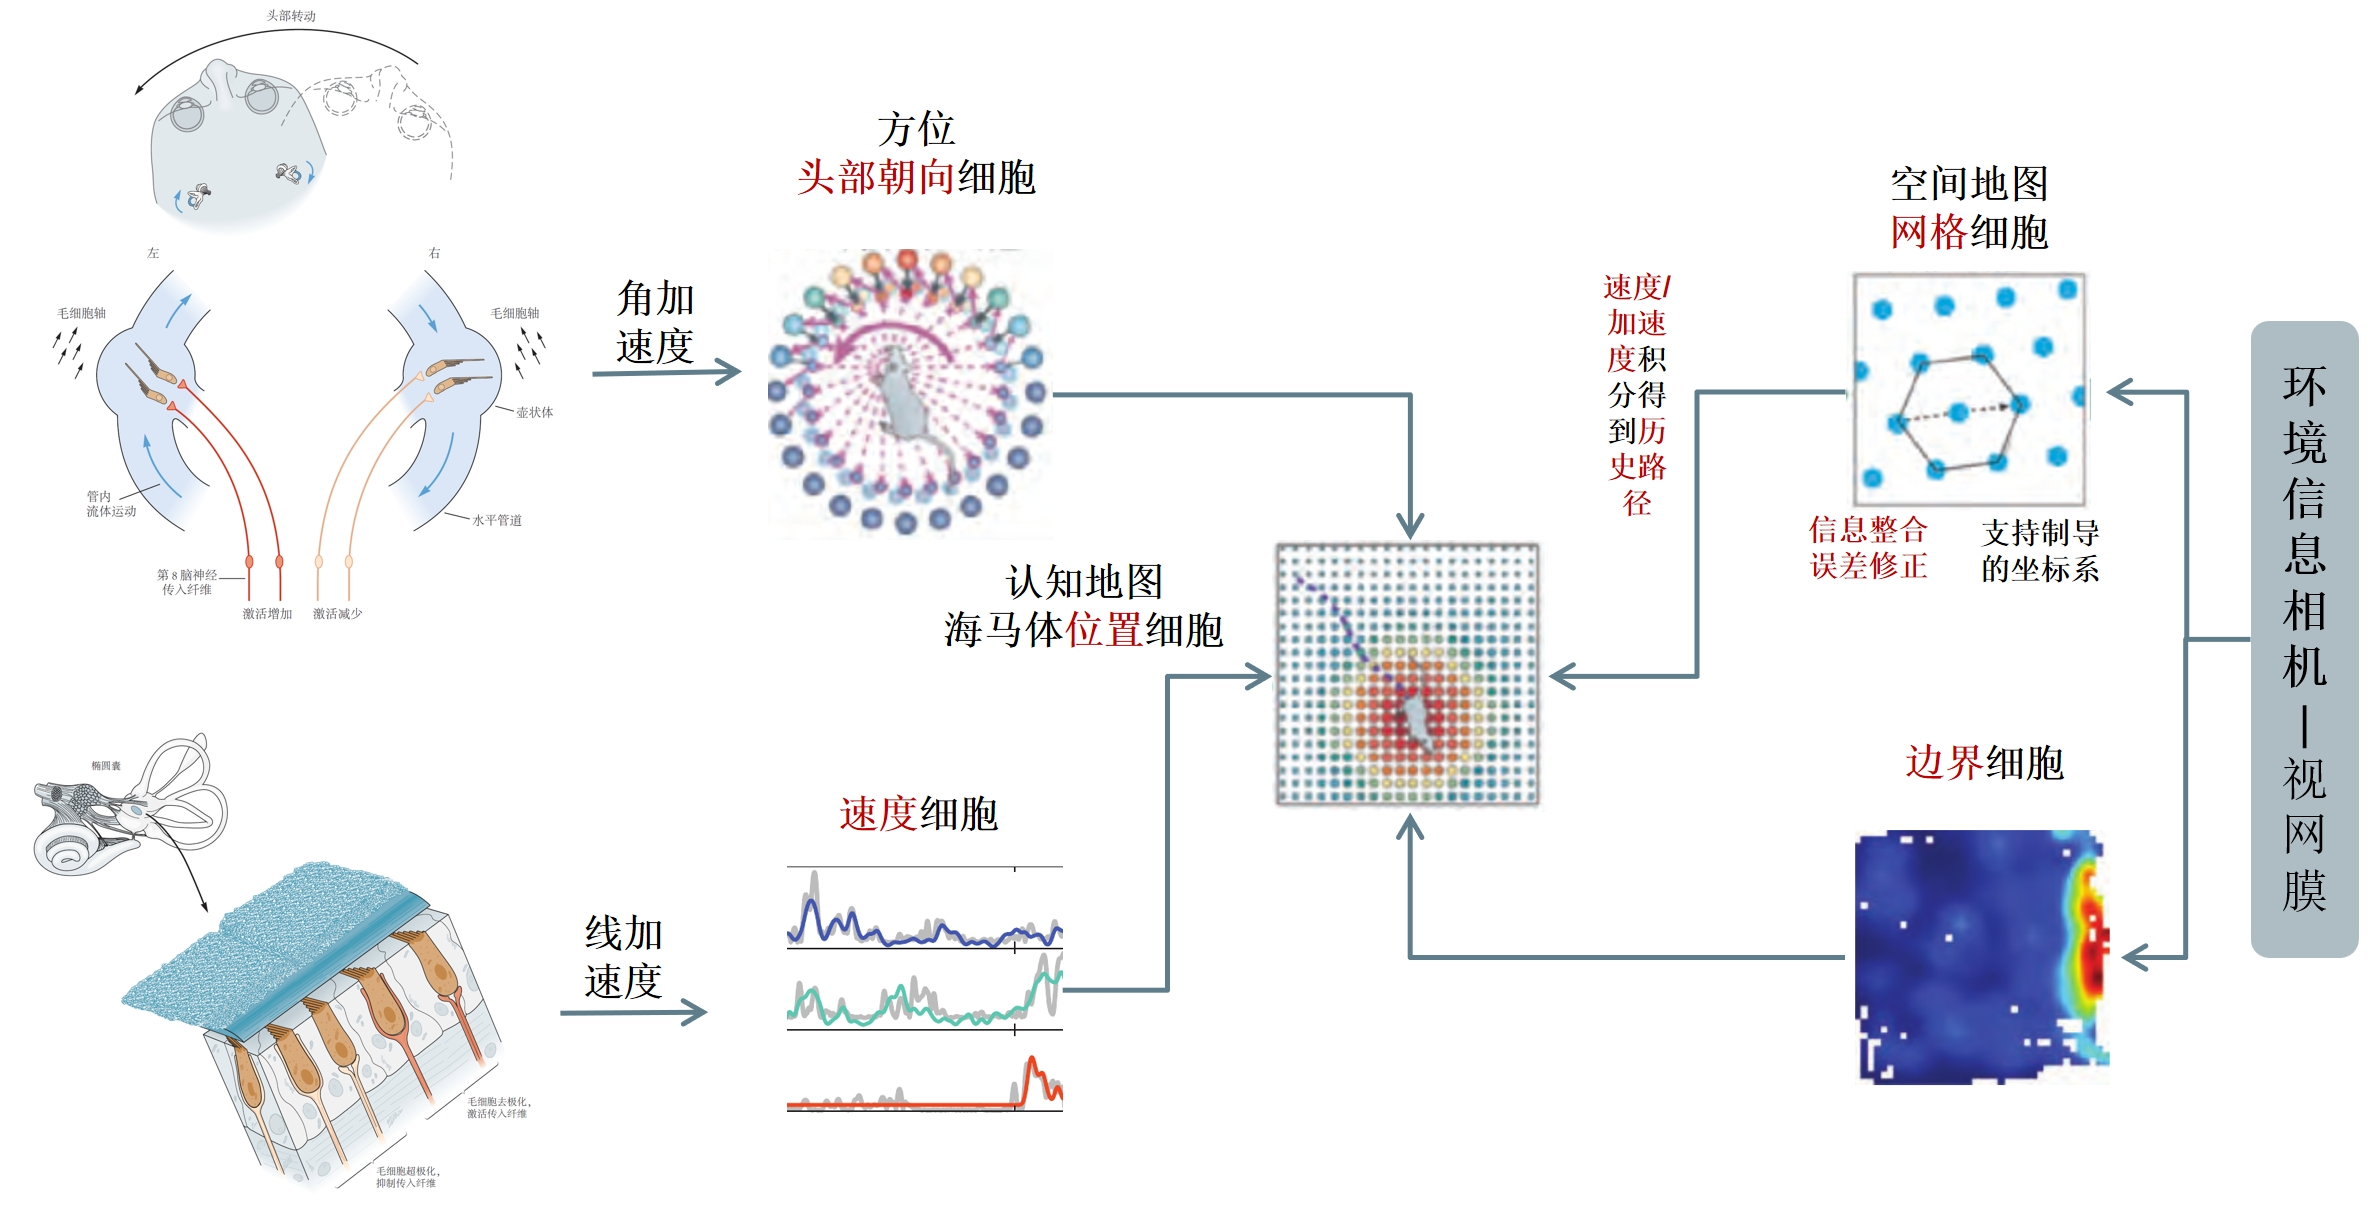
\includegraphics[width=\linewidth]{fig/pipeline.png}
	\caption{The network architecture of the BID agent is primarily composed of the perception network and the decision network.
		The perception module includes both the dorsal and ventral pathways, which allow the system to understand and process its surroundings.
		The decision network consists of five modules that represent different regions of the prefrontal cortex: the medial prefrontal cortex (MPC), orbital prefrontal cortex (OPC), caudal prefrontal cortex (CPC), dorsal prefrontal cortex (DPC), and ventral prefrontal cortex (VPC). 
		Specifically, the input to the system is an RGB image $f_{t} $, which represents the current visual scene.
		The output is the action $A_t$, which controls the ego-vehicle's maneuvering directly.
		The action $A_t$ includes the steering angle $ A_t^s $ and acceleration $ A_t^a $ of the vehicle, making BID a brain-inspired and end to end autonomous driving model.
		Besides, in the construction process of training dataset, the driving actions and input frames are paired.
	}
	\label{fig:fig2}
\end{figure*}


